\section{Results}
\subsection{Analog pixel circuit}
\subsubsection{Values and dimensions}
The transistor technology used limits the width to 

\begin{equation}
    \label{eq:limitsW}
    1.08 \mathrm{\mu m} \leq W \leq 5.04 \mathrm{\mu m}
\end{equation}

and limits the length to

\begin{equation}
    \label{eq:limitsL}
    0.36 \mathrm{\mu m} \leq L \leq 1.08 \mathrm{\mu m}.
\end{equation}

As explained in section \ref{sec:switch_dimensions}, the length and width of the switch transistors will be $1.08\mathrm{\mu m}$.

CS was tuned to $2 \mathrm{pF}$. The output from simulations with this value for the exposure-light corners min-min, min-max, max-min and max-max are shown respectively in figures \ref{fig:min-min}, \ref{fig:min-max}, \ref{fig:max-min} and \ref{fig:max-max}.

\begin{figure}
    \centering
    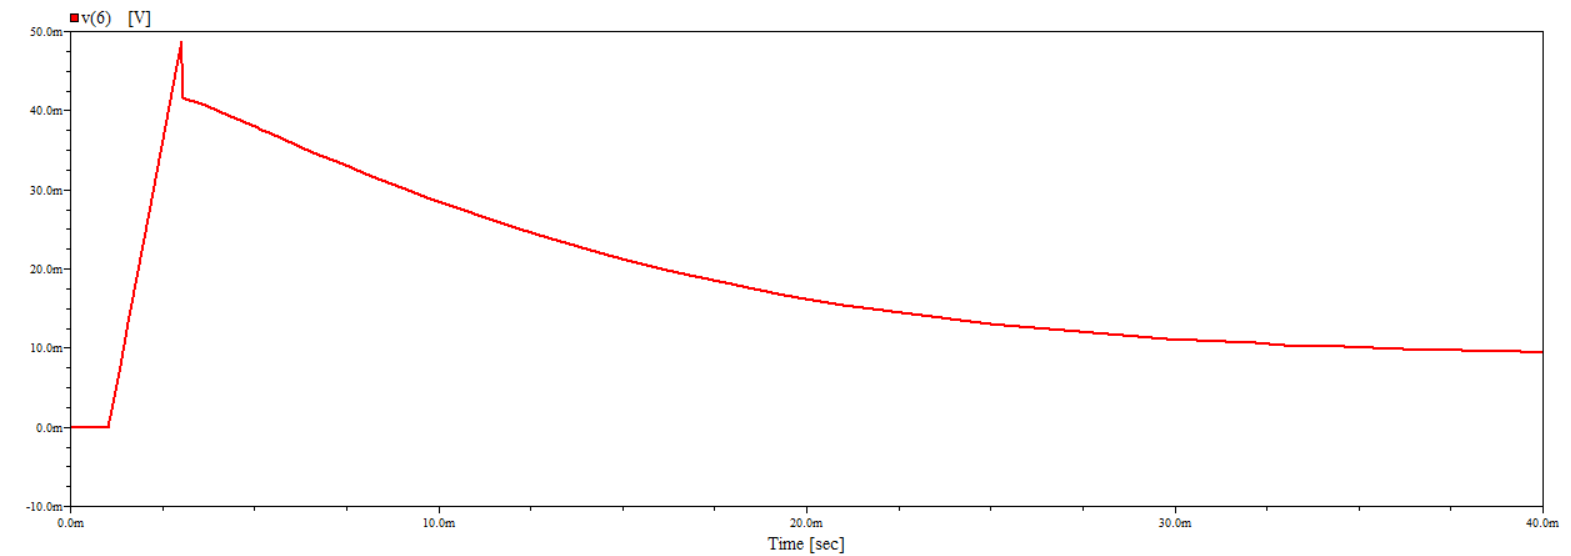
\includegraphics[width=\textwidth]{graphs/minExp_minLight.png}
    \caption{Minimum exposure time - minimum light}
    \label{fig:min-min}
\end{figure}

\begin{figure}
    \centering
    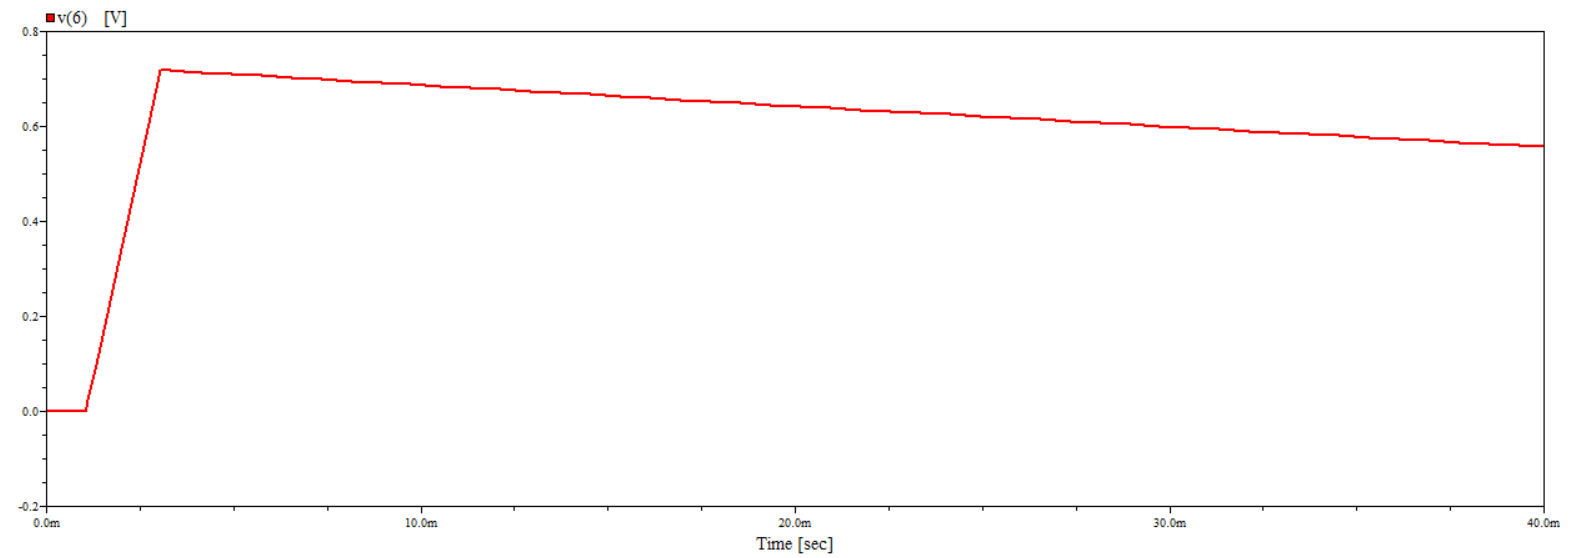
\includegraphics[width=\textwidth]{graphs/minExp_maxLight.png}
    \caption{Minimum exposure time - maximum light}
    \label{fig:min-max}
\end{figure}

\begin{figure}
    \centering
    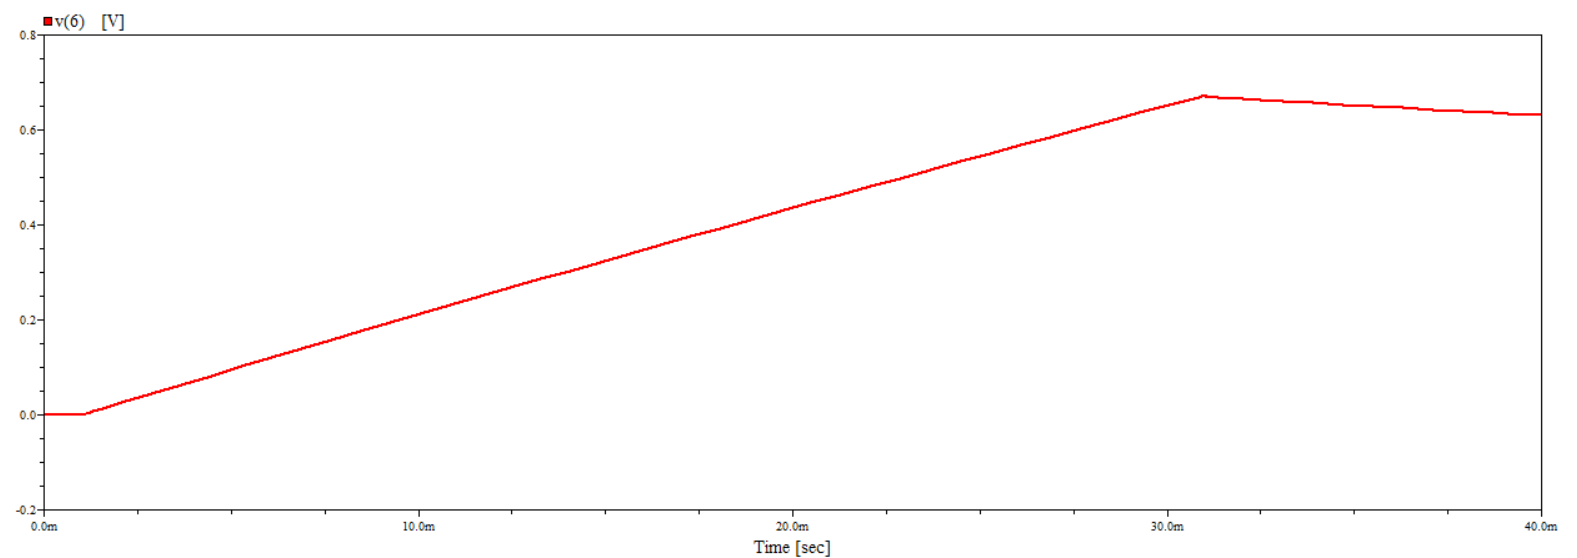
\includegraphics[width=\textwidth]{graphs/maxExp_minLight.png}
    \caption{Maximum exposure time - minimum light}
    \label{fig:max-min}
\end{figure}

\begin{figure}
    \centering
    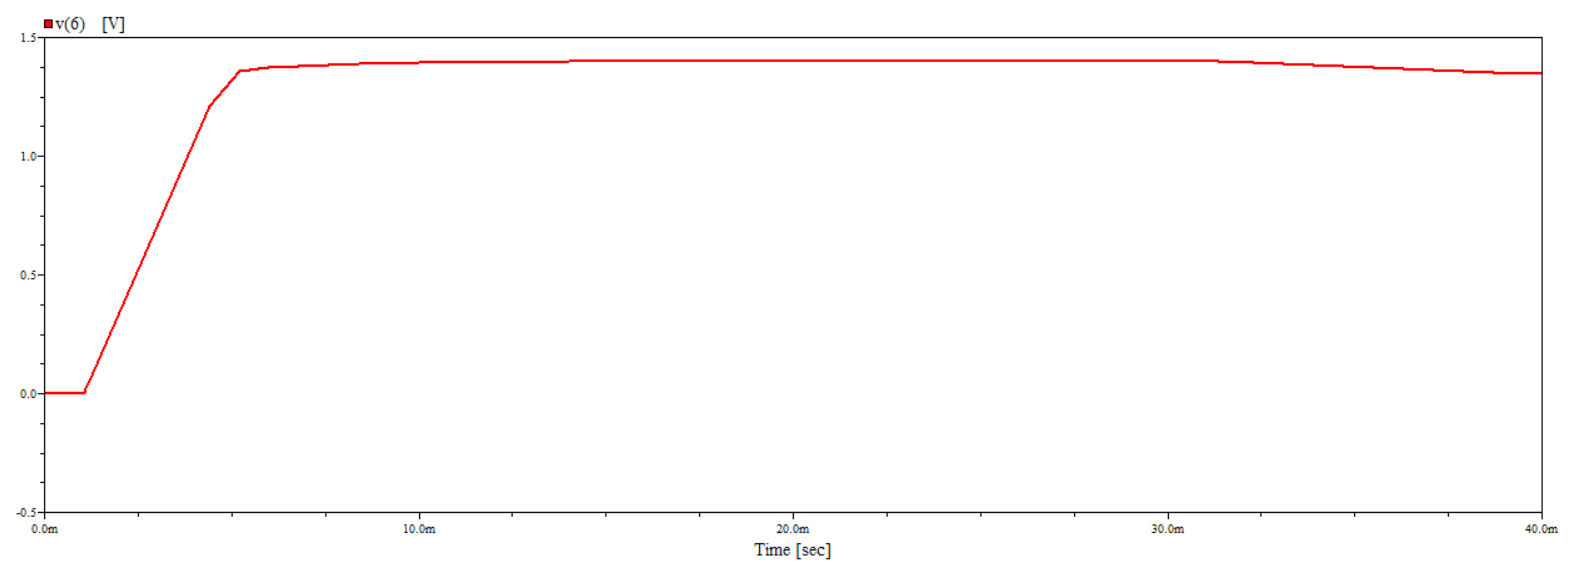
\includegraphics[width=\textwidth]{graphs/maxExp_maxLight.png}
    \caption{Maximum exposure time - maximum light}
    \label{fig:max-max}
\end{figure}

\subsubsection{Analog circuit simulation}

\subsection{Digital circuit}

\subsubsection{Digital circuit simulation}

Explaining the big waveform.

\begin{figure}
    \centering
    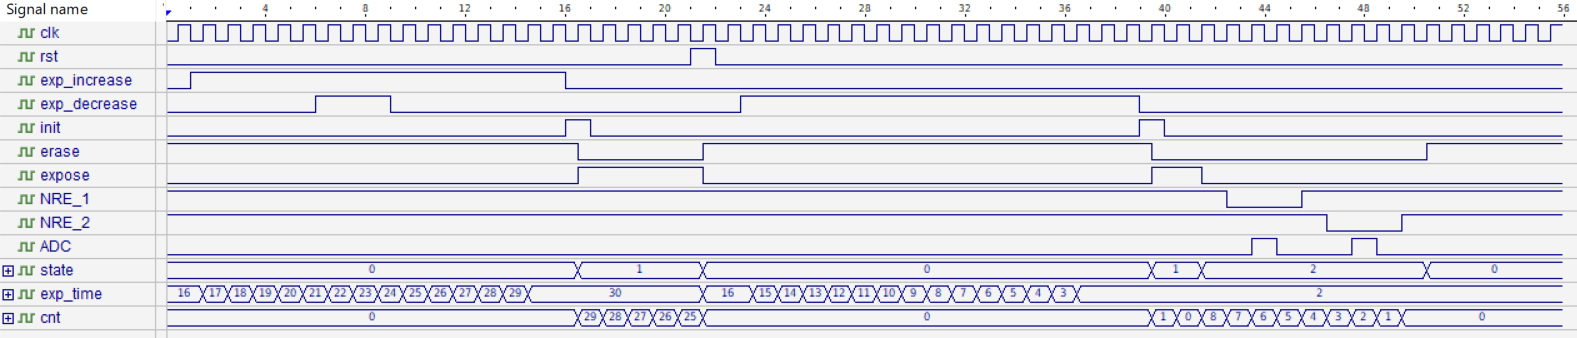
\includegraphics[width=\textwidth]{graphs/digital_waveform.png}
\end{figure}
